\chapter{Background}
\section{Switch Mode Power Supply}\label{section-smps}
The root of this approach is based on the electromagnetic interference (\acrshort{emi}) induced by switch mode power supplies (\acrshort{smps}). \cite{hesener2010electromagnetic,liu2002high} \acrshort{smps} is a solution proposed by electricians to have more efficient transformers because no current is dissipated as heat by going through resistors. One of its drawbacks is that it induces \acrshort{emi} on the electrical network and therefore to other appliances, possibly disturbing them. Actually, this drawback can be used to our advantage since each device emits a different \acrshort{emi} which could be seen as its signature. This comes from the fact that there are many types of \acrshort{smps}, including buck, boost, buck-boost, boost-buck, zeta, charge pump, flyback, RCC, Forward, push-pull and Ćuk. Of course, there are also many different needs in intensity and power for every appliance which make the signature a step further towards its uniqueness.


As an example one of the \acrshort{smps}, let's take the buck-boost. It is composed of one inductance, one capacitor, one diode, one switch (a transistor), and of course the voltage source and the load. On \autoref{fig:closed_buck-boost} we can see the buck-boost in its closed state. The part in red is the part where current is flowing: the voltage source is loading the inductance, while the capacitor is unloading into the target load. The voltage source can not induce anything in the right part of the schema because of the diode. When the inductance begins to be loaded enough, the voltage change opens the switch.
\begin{figure}[h]
    \centering
    \begin{circuitikz}[scale=2]
    \draw[color=red]
    (0,0) to[voltage source,i^>=$I_s$,v=$V_s$] (0,1)
          to[closing switch] (1,1)
          to[L] (1,0)
          -- (0,0);
    \draw
    (2,1) to[diode] (1,1)
    (2,0) -- (1,0);
    \draw[color=red]
    (2,0) to[C,i^<=$I_c$] (2,1)
          -- (3,1)
          to[generic,label=load,i^<=$I_{load}$,v_<=$V_{load}$] (3,0)
          -- (2,0);
    \end{circuitikz}
    \caption{Closed buck-boost}
    \label{fig:closed_buck-boost}
\end{figure}

We are then in the case shown on \autoref{fig:open_buck-boost}. Again, the part where the current flows is in red. Now, the inductance is unloading into the capacitor and the target load. The capacitor will then be able to be to unload again when the switch will be open.


\begin{figure}[h]
    \centering
    \begin{circuitikz}[scale=2]
    \draw
    (0,0) to[voltage source,i^>=$I_s$,v=$V_s$] (0,1)
          to[opening switch] (1,1)
    (1,0) -- (0,0);
    \draw[color=red]
    (1,1) to[L,i^>=$I_l$] (1,0)
    (2,1) to[diode] (1,1)
    (2,0) -- (1,0);
    \draw[color=red]
    (2,0) to[C,i_>=$I_l$] (2,1)
          -- (3,1)
          to[generic,label=load,i^<=$I_{load}$,v_<=$V_{load}$] (3,0)
          -- (2,0);
    \end{circuitikz}
    \caption{Open buck-boost}
    \label{fig:open_buck-boost}
\end{figure} %TODO sens des fleches ?

The percentage of time that the switch is open is called the duty cycle and controls the potential difference around the load. Because the power of the load may vary, the uptime and downtime are not the same for a fixed duty cycle and source voltage.

Every time the switch is opened or close, there are repercussions on the electrical network.

Also, because of regulations, appliances are equipped with \acrshort{emi} filters. Although they reduce the higher peaks, they also induce smaller variations in the EMI spectrum that make the EMI more unique for every appliance. This is again due to a lot of different filter types and their interactions with the \acrshort{smps}.



\subsection{Electromagnetic Interference}
\acrlong{smps} can induce electromagnetic interferences (\acrshort{emi}) by multiple means. The resistors affect the whole range of frequency, but capacitors and inductances mainly affect the higher frequencies, up to a few GHz.

Because not all the parts of appliances need the same input voltage, there could be multiple \acrshort{smps} inside an appliance. But even with only one \acrshort{smps}, the duty cycle of the converter coupled with the type of converter and the power of the appliance unload very different \acrshort{emi} on the network.


Also, no capacitor is ideal, there are equivalent series resistance (\acrshort{esr}) and inductance (\acrshort{esl}) used to represent it. When current goes through the \acrshort{esr}, there is a voltage drop delayed by the inductance. %TODO is that true? 
This has an effect on the network as well.
\begin{figure}[h]
    \centering
    \begin{circuitikz} \draw
    (0,0) to[R,label=ESR,o-] (2,0) to[L,label=ESL] (4,0) to[C,-o] (6,0);
    \end{circuitikz}
    \caption{Circuit model of non ideal capacitor}
    \label{fig:non_ideal_capacitor}
\end{figure}




\section{Fourier Transform}\label{section:ft}
The Fourier transform (\acrshort{ft}) is a way to represent a function of time into a function of frequencies. It exists for both continuous and discrete functions but as we are reading discrete values, we will focus on the discrete transform.
\begin{equation}S[k] = \sum_{n=0}^{N-1}s[n]e^{\frac{n-2i\pi k}{N}} \qquad \text{for}~0 \leq k < N\end{equation}
Where $N$ is the number of readings of the input signal, the upper case letter ($S$ in this case) is representing the function of frequency, and the lower case letter ($s$ in this case) is representing the function of time.

The inverse is 
\begin{equation} s[k] = \frac{1}{N}\sum_{n=0}{N-1}S[n]e^{\frac{2i\pi kn}{N}}  \qquad \text{for}~0 \leq k < N\end{equation}


When a signal $x[n] = \sum_{k=-\infty}^{+\infty}x[k]\delta[n-k]$ goes through a system $H[h]$, the output $y[n]$ is
\begin{equation}
\begin{array}{rl}
y[n] & = \displaystyle H\{x[n]\}\\
     & = \displaystyle H\{\sum_{k=-\infty}^{+\infty}x[k]\delta[n-k]\} \\
     & = \displaystyle \sum_{k=-\infty}^{+\infty}x[k]H\{\delta[n-k]\} \\
     & = \displaystyle \sum_{k=-\infty}^{+\infty}x[k]h[n-k] \\
\end{array}
\end{equation}
\myequations{Signal through a system}


\subsection{Nyquist-Shannon}\label{section:nyquist}
The Nyquist-Shannon theorem states that in order to not have aliasing in the signal we are processing, the sampling rate must be more than twice the highest frequency of the decomposition of the signal.

This means that if a signal is composed of frequencies higher than the half of the sampling frequency, there will be noise in the signal and the reproduction of a sampled signal would not result in the original signal. As an example, lets take \autoref{fig:nyquist-shannon}. You can see the 3 graphs on the left with 3 different sampling and on the right their respective \acrlong{dft}. The original function is $$f(t) = 1\sin(2\pi60.t) + 0.7\sin(2\pi110.t+5) + 1.2\sin(2\pi256.t)$$. On the first plot, we used a sampling frequency of 800Hz, and on the second and third plot a sampling frequency of 240Hz, the difference between those two that the latter has a shift of 2.0833ms in the sampling. The above sampling has a frequency of more than twice the highest frequency of the function $f(t)$, so there are indeed no problems with the \acrshort{dft}. But the two last sampling have a sampling frequency below the highest frequency so the result of the \acrshort{dft} might not be what we wanted. The amplitude for the 60Hz and the 110Hz components of the wave are correct but there is a component at around 18Hz that wasn't part of the original function.

Note that the inverse \acrshort{dft} don't produce the same function when there is a shifting in the sampling, even though the real part of the \acrshort{dft} is the same, because the imaginary part (not represented) changes the phase of the different component of the function.

The good thing is that the shifting doesn't change the value of the real part of the \acrshort{dft}, in most of the cases, even though the values we get are false.

But in most of the cases means “not all the cases”. On \autoref{fig:nyquist-shannon-2}, the parameters of sampling is the same, but the function has changed. It is now $$f(t) = 1\sin(2\pi60.t) + 0.7\sin(2\pi110.t+5) + 1.2\sin(2\pi300.t)$$. You can see that the higher frequency added up on the readings of 60Hz of the second samling parameters, but did the opposite on the third sampling parameters.


\begin{figure}
    \centering
    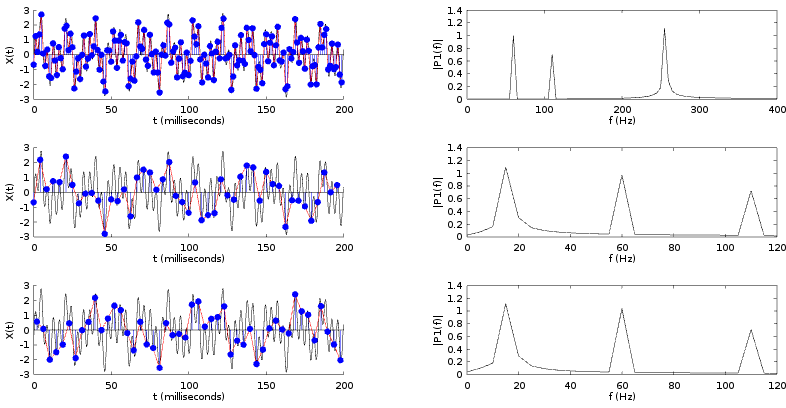
\includegraphics[width=\textwidth]{img/nyquist-shannon.png}
    \caption{Example of higher frequencies messing up the DFT}
    \label{fig:nyquist-shannon}
\end{figure}

\begin{figure}
    \centering
    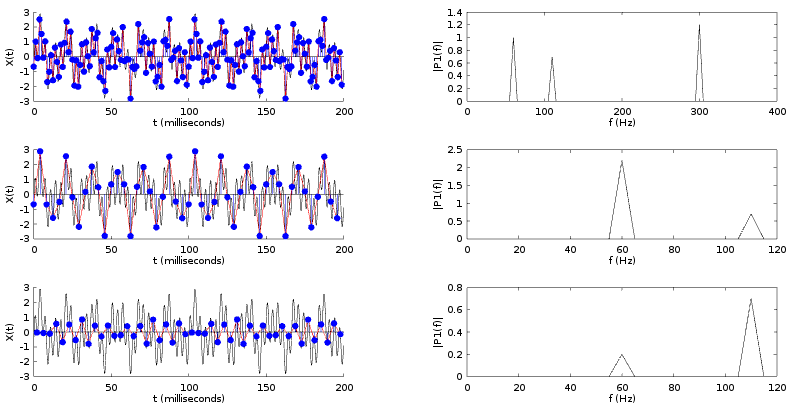
\includegraphics[width=\textwidth]{img/nyquist-shannon-2.png}
    \caption{Another example of higher frequencies messing up the DFT}
    \label{fig:nyquist-shannon-2}
\end{figure}


\subsection{Linear Time Invariant}
Most of the properties described below are true only in linear and time-invariant systems (\acrshort{lti}). If one of those two properties are not satisfied, it is harder or impossible to have a description of the system using Fourier Transforms. Electrical components can be well represented as a \acrshort{lti} system although a perfect \acrshort{lti} system doesn't exist. A resistor or other components' values are a function of the temperature, which is a function of the time. However, using \acrshort{lti} system theory on electrical systems works really good in practice because the variations of the values are expected to be very small.

\subsection{Properties}
The Discrete Fourier Transform (\acrshort{dft}) has a lot of properties but only the ones interesting fir this thesis will be discussed here.
\subsubsection{Linearity}
The response of a system to a sum of multiple signals is the sum of the responses of each individual signal :
\begin{equation}
\begin{array}{rl}
y(t) & = \displaystyle H\{\sum_{i=1}^{N}a_ix_i(t)\} \\
     & = \displaystyle \sum_{i=1}^{N}a_iH\{x_i(t)\} \\
     & = \displaystyle \sum_{i=1}^{N}a_iy_i(t)
\end{array}
\end{equation}
\myequations{Response of a sum of signals}

\subsubsection{Product and convolution}
The convolution of two functions is 
\begin{equation}f(t)*g(t)=\int_{-\infty}^{+\infty}f(\tau)g(t-\tau)d\tau\end{equation}\myequations{Convolution in continuous time}
and in discrete time and frequency :
\begin{equation}f[n]*g[n]=\sum_{k=-\infty}^{+\infty}f[k]g[n-k]\end{equation}\myequations{Convolution in discrete time}

The product in one domain is the convolution in the other domain. In continuous and discrete time respectively, we have
\begin{equation}
    y(t)=x(t)*h(t) \iff Y(j\omega) = X(j\omega)H(j\omega)
\end{equation}

\begin{equation}
    y[n]=x[n]*h[n] \iff Y(e^{j\Omega}) = X(e^{j\Omega})H(e^{j\Omega})
\end{equation}

\subsection{Differentiation}
\begin{equation}
\begin{array}{rl}
x(t)             & = \displaystyle \frac{1}{2\pi}\int_{-\infty}^{+\infty}X(j\omega)e^{j\omega t}d\omega \\
\frac{d}{dt}x(t) & = \displaystyle \frac{1}{2\pi}\int_{-\infty}^{+\infty}X(j\omega)\frac{d}{dt}e^{j\omega t}d\omega \\
                 & = \displaystyle \frac{1}{2\pi}\int_{-\infty}^{+\infty}X(j\omega)j\omega e^{j\omega t}d\omega \\
                 & = j\omega x(t)
\end{array}
\end{equation}

\subsubsection{Shifting}
One interesting property of the \acrshort{ft} is that the result of 

\subsection{Fourier transform in a system}\label{section:fourier-system}
As an example, lets take the simple system described on \autoref{fig:fft_system}\cite{LFSAB1106} :
\begin{figure}
    \centering
    \begin{circuitikz} \draw
    (0,0) to[voltage source,,v=$x(t)$] (0,2) to[R,label=R] (2,2) to[L,label=L] (4,2) to[C,label=C,i=$y(t)$] (4,0) to[] (0,0);
    \end{circuitikz}
    \caption{Simple LRC circuit}
    \label{fig:fft_system}
\end{figure}
Where $x(t)$ is the applied tension and $y(t)$ is the current. We have then
\begin{equation}L\frac{d^2y(t)}{dt^2} + R\frac{dy(t)}{dt}+\frac{1}{C}y(t) = \frac{dx(t)}{dt}\end{equation}\myequations{LRC system input-output relation}
and
\begin{equation}H(j\omega) = \frac{j\omega}{L(j\omega)^2+Rj\omega+\frac{1}{C}}\end{equation}\myequations{LRC system response}

Of course, this is in continuous times and we are measuring on a discrete interval. But this shows that even for a simple system the current flowing 
